\documentclass[a4paper,12pt]{article}
\usepackage[utf8]{inputenc}
\usepackage[english]{} % Sets the language
\usepackage[margin=2cm]{geometry} % Sets the margin size
\usepackage{graphicx} % Enhanced package for including graphics/figures
\usepackage{float} % Allows figures and tables to be floats
\usepackage{amsmath} % Enhanced math package prepared by the American Mathematical Society
\usepackage{amssymb} % AMS symbols package
\usepackage{bm} % Allows you to use \bm{} to make any symbol bold
\usepackage{verbatim} % Allows you to include code snippets
%\usepackage{setspace} % Allows you to change the spacing between lines at different points in the document
%\usepackage{parskip} % Allows you alter the spacing between paragraphs
\usepackage[version=3]{mhchem}
\usepackage{cite}
\usepackage{multicol,caption}
\usepackage{enumitem}
\usepackage{tabularx}
\usepackage{setspace}
\newenvironment{Figure}
  {\par\medskip\noindent\minipage{\linewidth}}
  {\endminipage\par\medskip}


\title{Final Project Report: 2D Diffusion Solver}
\author{Harrison Agrusa}


\begin{document}
\maketitle
\onehalfspacing
\section{Introduction}
In this paper I present my 2D diffusion solver. In Section \ref{math} I present the mathematical derivation of the 2D diffusiton equation. The algorithms used to solve the system is detailed in Section \ref{algorithms}. Section \ref{code use} discribes how the code is used, issues with the code, and opportunities for improvement. Finally, in Section \ref{test problem} I present a simple test problem and discuss how well the code works.


\section{Mathematics}\label{math}
Most of the information in this section is taken from \cite{slaybaugh}.\\
I am solving the time independent diffusion equation:

\begin{equation}
-\nabla \cdot D(\vec{r})\nabla\phi(\vec{r}) + \Sigma_{a}(\vec{r})\phi(\vec{r}) = S(\vec{r}) + v\Sigma_{f}(\vec{r})\phi(\vec{r})
\end{equation}
Where D is the diffusion coefficient, $\Sigma_{a}$ is the absorption cross-section, S is the neutron source term, v is the neutron velocity, and $\Sigma_{f}$ is the macroscopic fission cross-section. Note that D, $\Sigma_{a}$, and $\Sigma_{f}$ are spacially dependent, as there can be multiple materials in our system.

In 2-D this equation takes the following form:

\begin{equation}
    -\frac{\partial}{\partial x}D(x,y)\frac{\partial}{\partial x}\phi(x,y) - \frac{\partial}{\partial y}D(x,y)\frac{\partial}{\partial y}\phi(x,y) + \Sigma_{a}(x,y)\phi(x,y) = S(x,y) + v\Sigma_{t}(x,y)\phi(x,y)
\end{equation}

When we discritize this equation, we assume that D, $\Sigma_{a}$, and $\Sigma_{f}$ are cell-centered and constant throughout each cell. S and $\phi$ are edge-centered quantities, meaning they are only explicitly defined at the interface between two cells. Then we can represent all of these quantities with 2D arrays, using indexes i and j to reference the x and y directions, respectively. For example $D(x,y)$ becomes $D_{i,j}$ over the interval $[x_{i-1},x_{i}]$ and $[y_{i-1},y_{i}]$. For edge-centered values like $\phi(x,y)$, we call it $\phi_{i,j}$ at the point $(x_{i},y_{i})$ and must interpolate to find it at positions other than the cell edges. \\

To solve for $\phi(x,y)$, we effectively want to do a volume integral over entire diffusion equation. This means we need to find ways to integrate each term, then put it in a matrix form to solve.
\begin{equation}
    \int_{V}d\vec{r}\big[ -\nabla \cdot D(\vec{r})\nabla\phi(\vec{r}) + \Sigma_{a}(\vec{r})\phi(\vec{r}) - v\Sigma_{t}(\vec{r})\phi(\vec{r})= S(\vec{r})
\big]
\end{equation}

Where the volume integral is really just an integral over area because we are working in 2D. To solve the first term (Streaming Term), we use Gauss' Theorem to turn it into a surface integral:
\begin{equation}
    \int_{V}d\vec{r}\big[ -\nabla \cdot D(\vec{r})\nabla\phi(\vec{r})\big] = -\int_{S}d\vec{S}\cdot\big[ D(\vec{r})\nabla\phi(\vec{r})\big] = -\int_{S}d\vec{S}D(\vec{r})\frac{\partial}{\partial\hat n}\phi(\vec{r})
\end{equation}
Because of the dot product, we know that the only terms that contribute to the integral will be those where the direction of the partial derivatve is perpendicular to the surface.

This code will use constant mesh sizes, $\delta$ and $\epsilon$, that refer to the size of the mesh in the x and y directions, respectively.

For the surface above the cell (i,j),:
\begin{equation}
    \frac{\partial}{\partial \hat n}\phi(\vec{r}) = \frac{\partial}{\partial \hat y}\phi(\vec{r}) = \frac{\phi_{i,j+1} - \phi_{i,j}}{\epsilon}
\end{equation}
For the surface to the right of cell (i,j):
\begin{equation}
     \frac{\partial}{\partial \hat n}\phi(\vec{r}) = \frac{\partial}{\partial \hat x}\phi(\vec{r}) = \frac{\phi_{i+1,j} - \phi_{i,j}}{\delta}
\end{equation}
The same logic is used for the integral over the surfaces to the left and bottom of cell (i,j).

Therefore, the streaming term for the top surface is:
\begin{equation}
    -\int_{top}d\vec{S}D(\vec{r})\frac{\partial}{\partial \hat n}\phi(\vec{r}) = \frac{\phi_{i,j+1} - \phi_{i,j}}{\epsilon} \bigg(\frac{D_{i,j+1}\delta + D_{i+1,j+1}\delta}{2}\bigg)
\end{equation}
The factor of 2 is because $D_{i,j}$ is a cell-centered value and $\phi_{i,j}$ is edge-centered, so we have to take an average to get the edge-centered value for $D_{i,j}$. We do the same thing for the surfaces to the left, right, and bottom of the cell we are concerned with. Adding all of these terms gives us the full streaming term.

Next, we need to solve the absorption term. Because the absorption term is cell-centered and the neutron flux is edge-centered, we compute integrals over four different sub-volumes:

\begin{equation}
    \int_{x}\int_{y}dxdy\Sigma_{a}(x,y)\phi(x,y) = \phi_{i,j}\bigg(\Sigma_{a, i,j}V_{i,j} + \Sigma_{a, i+1,j}V_{i+1,j} + \Sigma_{a, i,j+1}V_{i,j+1} + \Sigma_{a, i+1,j+1}V_{i+1,j+1} \bigg)\equiv \bf{\Sigma_{a,i,j}}
\end{equation}
 Where each subvolume term, $V_{i,j}$, is the subvolume we integrated. Adding each volume term gives the total volume of a vell. Because $\delta$ and $\epsilon$ are constant throughout the mesh, each subvolume term is conveniently the identical - just 1/4 the volume of a cell. So,
 \begin{equation}
     V_{i,j}=V_{i+1,j}=V_{i,j+1}=V_{i+1,j+1} = \frac{1}{4}\delta\epsilon
 \end{equation}

 We treat the fission term just like the absorption term:

 \begin{equation}
    -\int_{x}\int_{y}dxdy\Sigma_{f}(x,y)\phi(x,y) = -\phi_{i,j}\bigg(\Sigma_{f,i,j}V_{i,j} + \Sigma_{f, i+1,j}V_{i+1,j} + \Sigma_{f, i,j+1}V_{i,j+1} + \Sigma_{f, i+1,j+1}V_{i+1,j+1} \bigg) \equiv \bf{\Sigma_{f,i,j}}
 \end{equation}

 Finally, we have the source term which we also treat like the previous two:
 \begin{equation}
     \int_{V}d\vec{r}S(\vec{r}) = \int\int dxdy S(x,y) = S_{i,j}V_{i,j} + S_{i,j+1}V_{i,j+1}+S_{i+1,j}V_{i+1,j} + S_{i+1,j+1}V_{i+1,j+1} \equiv \bf{S_{i,j}}
 \end{equation}


If we put all of these terms togehter for a given cell i,j we get the following difference equation:
\begin{equation}
    a_{i-1,j}^{i,j}\phi_{i-1,j} +
    a_{i+1,j}^{i,j}\phi_{i+1,j} +
    a_{i,j-1}^{i,j}\phi_{i,j-1} +
    a_{i,j+1}^{i,j}\phi_{i,j+1} +
    a_{i,j}^{i,j}\phi_{i,j} = S_{i,j}
\end{equation}
The top indices refer to the cell we are in and the bottom indices refer to a neighboring cell that is coupled to the cell we are in. For example, $a_{i-1,j}^{i,j}$ tells us how much the flux of the cell to the left should influence the cell we are in.
If we collected all of these terms for each of our $i\times j$ cells, we can construct a $(i+1)\times(j+1)$ matrix of $(i+1)\times(j+1)$ matrices. Solving this system of matrices will give us the solution we are looking for - $\phi(x,y)$.

The only information required to solve the equation is boundary conditions. We treat the left and bottom faces (in addition to top left and bottom right corners) as a vacuum. This means that $\phi = 0$ at these locations. For vacuum boundaries, have 2 and 3-point difference equations for corners and sides, respectively. This is because we drop the $a_{i\pm1, j\pm1}^{i,j}$ terms that are outside of the problem boundaries and set $\phi_{boundary}$ equal to zero.

The top and right faces are reflecting boundaries meaning that must satisfy the condition of zero net current at the boundary:
\begin{equation}
    \frac{d}{d\vec{r}}\phi(\vec{r})|_{boundary} = 0
\end{equation}
This means we only integrate the equation over the subvolumes that are still within the boundary of the problem, yielding a 4-point difference equation.

With the boundary conditions known, we must implement an algorithm to solve our matrix.


\section{Algorithms}\label{algorithms}
We have a system of equations of the form
\begin{equation}
    \bf{A}\bf{x} = \bf{b}
\end{equation}

where {\bf A} is a matrix containing all of the $a_{i\pm1, j\pm1}^{i,j}$ entries from the difference equations, {\bf x} is a 1 dimensional matrix of length $n\times m$ containing $\phi$, and {\bf b} is another 1D matrix containg the source terms. {\bf A} has shape $(n\times m)\times (n\times m$)) where n and m are the number of nodes in the x and y directions respectively. Being such a massive matrix, this is nearly impossible to solve using directed methods. Therefore we will use Successive Over-Relaxation (SOR)\cite{Hadjidimos2000177}, an iterative method of solving this system. Although the equation for this algorithm looks complicated it is quite simple. Mathematically, the SOR method looks like the following:

\begin{equation}\label{SOR}
    x_{i}^{k+1} = (1-\omega)x_{i}^{k} + \frac{\omega}{a_{ii}}\bigg(b_{i} - \sum_{j<i}a_{i,j} x_{j}^{k} - \sum_{j>i}a_{i,j}x_{j}^{k}\bigg)
\end{equation}

$x_{i}^{k}$ is the (k+1) guess of ith element $x_{i}^{k}$ is the kth guess of the ith element of the vector {\bf x}. $a_{i,i}$ denotes the ith diagonal of the matrix {\bf A} and $a_{i,j}$ is the i,j matrix element. $b_{i}$ is the ith element of {\bf b}. Finally $\omega$ is the relaxation factor, a number between 0 and 2.

In slightly simpler terms, we start with an itinial guess for {\bf x}. We can call it { $\bf x^{0}$ } We then iterate the entire {\bf A} matrix (over i and j) and update the ith element of $\bf x^{0}$ based on Equation \ref{SOR}. It is important to note that when we are update element $x_{i}^{k+1}$, we use that new value when updating the next element, $x_{i+1}^{k+1}$.


\section{Code Use}\label{code use}
The code structure is fairly straight forward. The input deck is itself a python script, just like all of the other scripts used in this code. In the input deck, you specify the parameters of the problem such as the cell sizes, and number of cells. 2D arrays containing the diffusion constant, absorption and fission cross sections and source terms are also constructed in the input deck. The only requirement is that they are of the correct dimensions. This is all explained in the sample input deck ``sample\_deck.py''. The input deck uses the solver() function from the script ``main.py'' to solve the problem. This routine constructs the matrices {\bf A} and {\bf b} using functions from the script ``construct.py''. It then calls the SOR() function that is located in the file ``SOR.py''. This function returns the solution (a 1D vector), the number of iterations to reach the solution, and the relative error of the solution. Once this information is returned to the input deck script, one can reshape the solution vector into a 2D array for plotting using the x\_to\_phi() function in ``construct.py''. Then, the user can use the premade functions in ``make\_plots.py'' to plot a 2D contour plot, or a 3D surface plot. ``make\_plots.py'' also contains functions that are useful for finding the optimal $\omega$ and for exploring scaling relationships between the resolution and the time and number of iterations required to solve.

There are several issues with this code in its current form, most of which probably only require a few more hours of work and/or the eyes of a more skilled coder. First, this code only works with reflecting boundary conditions on all sides. For some reason, I can't get the vacuum boundary conditions to work - it is probably an easy fix if I had another set of eyes looking at the code. In the ``construct.py'' file, you can see how I set up the vacuum boundary conditions. I then override some of the matrix entries with a reflecting boundary condition. I did this so you can see what I was trying to do with the vacuum boundary. When I don't override things with a reflecting boundary condition, I end up creating a singular matrix which is unsolvable.

Additionally, the x and y dimension and cell size must be the identical. Given more time, I could easily have fixed this to make the code more robust.

The final issue is that it is burdensome to simulate a real system. To simulate real materials, you have to look up the diffusion constant, and absorption and fission x-sections  for the neutron energy in mind and calculate them by hand. If I had more time, I would have written a function that could compute these quantities from existing databases.


\section{Test problems}\label{test problem}
The primary problem that I tested was for a point source located in the middle of a 2x2 cm grid. The point source is $10^{9}$ neutrons/cm/s source of thermal neutrons (0.025 eV). The rest of the space is filled with water. The characteristics of the system are shown in Table \ref{test table}.

\begin{table}[h]
\begin{center}
Test Problem Parameters\\
\footnotesize
\begin{tabular}{c c}
\hline \hline
a, b & 1 cm\\
Source & $10^{9} \quad [cm^{-1}s^{-1}]$, 0.025 eV neutrons, Point Source\\
D & $0.142 \quad [cm]$ (water everywhere)\\
$\Sigma_{a}$ & $0.022 \quad [cm^{-1}]$ \\
$v$ & $2.2\times10^{5} \quad [cm s^{-1}$] Thermal neutron velocity\\
$\Sigma_{f}$ & 0 (approximation, $H_{2}O$ isn't going to fission)\\
\hline
\end{tabular}
\caption{\label{test table}}
\end{center}
\end{table}

After the test problem seemed to be working, ran it several times with different relaxation factors. At a cell size of 0.1 cm (20 cells in each direction for a total of 400 cells), I found an optimal relaxation factor of about 1.7 which is a bit higher than I expected. Figure \ref{optimal omega} shows the plot I made to find this optimal value. It is interesting that the time required to solve the system doesn't scale perfecly with the number of iterations. I have a feeling that this might be due to the fact that my computer was doing other tasks at the time, and not focused only on running this problem.

\begin{figure}
\centering
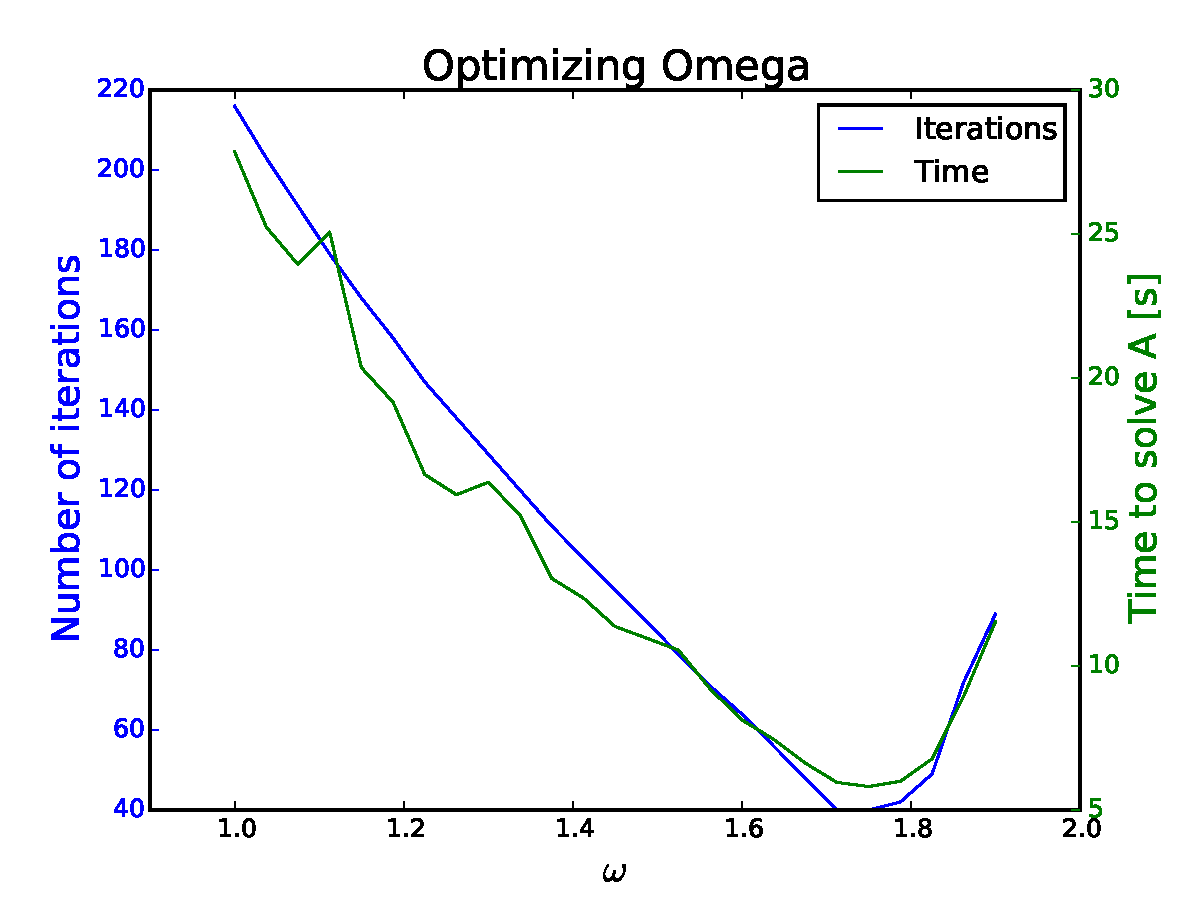
\includegraphics[width=.5\textwidth]{opt_omega_center_source.pdf}
\caption{\label{optimal omega} Plot of different relaxation factors and the number of iterations and time required to reach a relative error below $10^{-4}$}
\end{figure}

Figure \ref{contour plot} shows a contour plot of $\phi(x,y)$ at a cell resolution of 0.05 cm. The image is still rather grainy, yet it took my compute something like 10 minutes to solve!

\begin{figure}
\centering
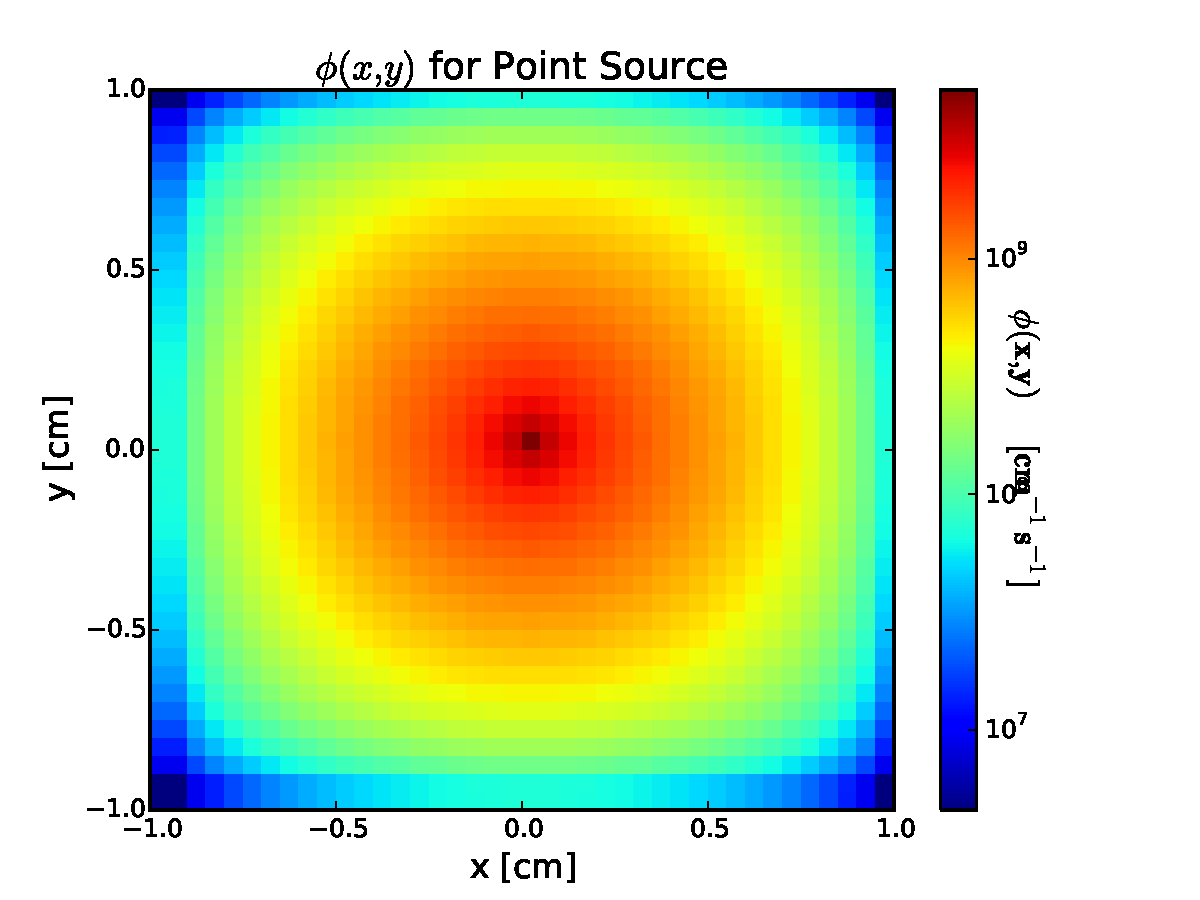
\includegraphics{point_source_2D_big.pdf}
\caption{\label{contour plot} Contour plot of $\phi(x,y)$ at a cell resolution of 0.05 cm.}
\end{figure}


\bibliographystyle{unsrt}%Used BibTeX style is unsrt
\bibliography{cite}













\end{document}